\chapter{Julia} \label{cap_julia}

\say{\textsf{Julia} es un lenguaje de programación gratuito y de código abierto desarrollado por Jeff Bezanson, Alan Edelman, Viral B. Shan y Stefan Karpinski en el MIT}, \cite{Hackers}.  Su propósito general es ser tan rápido como \textsf{C}, mientras mantiene la facilidad de lenguaje de \textsf{R} o \textsf{Python}. Es una combinación de sintaxis simple con alto rendimiento computacional. Su slogan es \say{\textsf{Julia} se ve como \textsf{Python}, se siente como \textsf{Lisp}, corre como \textsf{Fortran}}, \cite{Hackers}. 

La creación de \textsf{Julia} generó una gran impresión en la comunidad científica ya que busca resolver lo que se conoce como la \textit{Ousterhout's dichotomy} (la dicotomía de Ousterhout's). El problema establece que los lenguajes de programación se pueden dividir en dos categorías: programación de sistemas (\textit{system programming}) y lenguaje de secuencias de comandos (\textit{scripting languages}). Los lenguajes de la primera categoría tienden a ser difíciles de usar pero muy rápidos, mientras que los que forman parte de la segunda categoría son fáciles de usar pero lentos en ejecución. \textsf{Julia} busca tomar lo mejor de ambas categorías al implementar un conjunto de maneras en las que se logra una ejecución rápida de código con la sintaxis más sencilla posible. 

Por ejemplo, \textsf{Julia} tiene un compilador \textit{just in time (JIT)} lo que implica que \textsf{Julia} se compila al momento de la ejecución y guarda el código con los tipos de objeto que encuentra. Si el mismo código se ejecuta con objetos de diferente tipo, \textsf{Julia} recompila y guarda las instrucciones nuevas. Esto hace que el lenguaje no invierta tiempo en decidir el tipo de objeto con el que se está trabajando. Adicionalmente, el compilador \textit{JIT} tiene como consecuencia que la primera ejecución del código es considerablemente más lenta que las posteriores. Otro ejemplo es el uso de \textit{multiple dispatch} o dispatch múltiple del que se hablará más en la sección \ref{subMultipleDispatch}. Si se busca conocer más sobre las características de \textsf{Julia}, se recomienda ver la tesis de \cite{tesis_bezanson}. 

Esta combinación de características hace que \textsf{Julia} sea un lenguaje de programación que ha tomado fuerza  en la comunidad científica últimamente. Ya que es un lenguaje poco conocido, en esta sección se explica como instalar \textsf{Julia} en una computadora con sistema operativo \textsf{Windows} y algunos de los básicos del lenguaje.

\section{Reproducibilidad}
Antes de continuar, se enfatiza que esta tesis es completamente reproducible. Peng y Hicks del departamento de bioestadística en la Universidad John Hopkins definen \say{un análisis de datos publicado es reproducible si el conjunto de datos y el código utilizados para crear el análisis de datos está disponible para que otros lo analicen y estudien de manera independiente}, \cite{peng2021reproducible}. A pesar de que en el artículo enfatizan que esta definición puede ser un tanto ambigua, sí resaltan que la reproducibilidad es un medio para revisar y, posteriormente, confiar en el análisis de otros. 

Uno de los beneficios de tener un trabajo de investigación reproducible es que \say{los lectores obtienen los datos y el código computacional, los cuales son valiosos al grado de que pueden ser reutilizados o rediseñados para futuros estudios o investigaciones}, \cite{peng2021reproducible}. El código programado para esta tesis se encuentra en la plataforma de GitHub, específicamente en la liga \url{https://github.com/valperez/Tesis_Julia}. Los datos utilizados también se pueden encontrar en la liga anterior o en la fuente que se indica al mencionarlos. 

\section{Instalación}
Este trabajo se presenta como si se trabajara en un ambiente de \textsf{Windows}. La instalación y uso en los sistemas \textsf{Mac} y \textsf{Linux} es muy similar y no se mencionará.  

Al momento de la escritura de esta tesis la versión de \textsf{Julia} disponible es la \textsf{v1.7.3}. El primer paso es descargar \textsf{Julia} desde la página \url{https://julialang.org/downloads/}. 

Para el sistema operativo \textsf{Windows} se tiene la opción de un instalador de 64-bits o uno de 32-bits. El tipo de sistema que tiene un ordenador se verifica en \textsf{Start} $>$ \textsf{Configuración} $>$ \textsf{Sistema} $>$ \textsf{Acerca de}. Se debe seleccionar el \textsf{installer} y no el \textsf{portable}. Una vez descargado, se debe seleccionar el archivo \textsf{.exe} y seguir los pasos de instalación. 

\section{Símbolo del sistema}
Una vez instalado, se puede ejecutar \textsf{Julia} desde el símbolo del sistema o desde alguna interfaz gráfica como \textsf{Atom}, \textsf{Visual Studio Code} o \textsf{Jupyter Notebook}. De este último se presenta una explicación detallada en el capítulo \ref{cap_jupyter}. 

Una de las ventajas de utilizar \textsf{Julia} desde el símbolo del sistema (también conocido como \textit{Command Prompt} o \texttt{cmd}) es que se pueden controlar algunos parámetros del lenguaje. Mi sugerencia es que se comience a usar \textsf{Julia} directo desde la interfaz nativa. Posteriormente, cuando se entienda lo básico y los programas generados requieran un mayor nivel computacional, entonces se puede migrar a usar el \texttt{cmd} para correr \textsf{Julia}. 

\subsection{\textit{Multithreading}}
Una de las razones por la que \textsf{Julia} tiene gran velocidad es por su capacidad para multihilo (\textit{multithreading} en inglés). El multihilo es un tipo de paralelismo que utiliza \textsf{Julia} para ejecutar diferentes procesos de manera simultánea. Un proceso puede contener múltiples hilos donde cada hilo se ejecuta en un núcleo de la CPU. Los hilos comparten el espacio de memoria del proceso. 

La meta de los autores de \textsf{Julia} fue crear un lenguaje de programación con un rendimiento tan alto que pudiera ejecutar varias tareas de manera simultáneas. Debido a que uno de los objetivos de esta tesis es mostrar la eficiencia y velocidad de \textsf{Julia}, es crucial conocer la característica del \textit{multithreading} y cómo utilizarla. 

Si se está ejecutando \textsf{Julia} por medio del \texttt{cmd} es necesario modificar la cantidad de hilos que se va a utilizar antes de ejecutar \textsf{Julia}.  En \textsf{Windows}, esto se modifica con el comando \texttt{set Julia\_NUM\_THREADS=4} \citep{manual_Julia}. Si se está trabajando con otro sistema operativo, la página \url{https://docs.julialang.org/en/v1/manual/multi-threading/}
puede ser una guía para modificar la cantidad de hilos. En este ejemplo se cambiaron los hilos a 4, pero se puede asignar cualquier número. Sin embargo, se recomienda que éste no exceda de la cantidad de procesadores lógicos de la computadora.  

Si se está usando \textsf{Julia} en algún otro entorno de programación la modificación del número de hilos se hace de forma diferente. Cada programa tiene su manera de hacerlo y usualmente las instrucciones vienen en el manual del mismo. Para observar que el cambio se ejecutó de manera correcta (independientemente del editor de texto elegida) basta con correr el comando \texttt{Threads.nthreads()} y observar que la respuesta sea el número deseado.

\section{Básicos de Julia}
\say{Como el compilador de \textsf{Julia} es diferente a los intérpretes usados para lenguajes como \textsf{Python} o \textsf{R} se puede percibir que el funcionamiento de \textsf{Julia} no es intuitivo en un principio. Una vez que se entienda como funciona \textsf{Julia}, es fácil escribir código que es casi tan rápido como \textsf{C}}, \cite{manual_Julia}. En esta sección se presenta una introducción a la sintaxis del lenguaje que se tomó del manual oficial de \textsf{Julia}, \cite{manual_Julia}. 

La asignación de variables se hace con un signo de igualdad $=$. El ejemplo más sencillo de esto es ejecutar 
\begin{minted}{julia}
	julia> x = 2
	2
\end{minted}

\noindent donde se asigna a x el valor de 2. 

\subsection{Operaciones matemáticas básicas}
La tabla \ref{operaciones_basicas_julia} muestra la sintaxis usada para las operaciones matemáticas básicas en \textsf{Julia}. Los operadores están definidas para objetos de tipo numérico como \texttt{Float64} e \texttt{Int8}. 

\begin{center}
	\begin{longtable}{|c|c|c|} 
		\hline
		Expresión & Nombre & Descripción \\ 
		\hline 
		\texttt{+x} & suma unaria & la operación identidad \\ 

		\texttt{-x} & resta unaria & asigna a los valores sus inversos aditivos \\ 

		\texttt{x + y} & suma binaria & realiza adición \\ 

		\texttt{x - y} & resta binaria & realiza sustracción \\

		\texttt{x * y} & multiplicación & realiza multiplicación \\

		\texttt{x / y} & división & realiza divisiones \\

		\texttt{x $\div$ y} & división de enteros & $x / y$ truncado a un entero \\

		\texttt{x $\setminus$ y} & división inversa & equivalente a dividir \texttt{y / x} \\

		\texttt{x $\wedge$ y} & potencia & eleva \texttt{x} a la potencia \texttt{y} \\

		\texttt{x \% y} & residuo & equivalente a \texttt{rem(x,y)} \footnote{La operación \texttt{calcula el módulo entre \texttt{x} y \texttt{y}}} \\
		
		\texttt{!x} & negación & realiza lo contrario de \texttt{x} \\
		
		\texttt{x \& \& y} & \textit{and} lógico & verifica si \texttt{x} y \texttt{y} se cumplen \\
		
		\texttt{x || y} & \textit{or} lógico & verifica si al menos uno, \texttt{x} o \texttt{y},  se cumplen \\
		\hline
	\end{longtable} 
	\captionof{table}{Operaciones básicas en Julia} \label{operaciones_basicas_julia}
\end{center}


\subsubsection{Operaciones básicas en vectores}
En \textsf{Julia} cada operación binaria tiene su correspondiente operación punto (\textit{dot operation} en inglés). Estas funciones están definidas para efectuarse elemento por elemento en vectores y matrices. Para ejecutarlas basta agregar un punto antes del operador binario. Por ejemplo,

\begin{minted}{julia}
	julia> [1 9 9 7] .^ 2
	1x4 Matrix{Int64}:
	1 81 81 49
\end{minted}

 \noindent eleva cada uno de los elementos del vector al cuadrado. 

\textsf{Julia} maneja los números imaginarios utilizando el sufijo \texttt{im}. Sin embargo, no se utilizaron en este trabajo así que se omitirá dar mayor explicación. 

\subsection{\textit{Strings} (secuencias de caracteres)} 

Además de números, \textsf{Julia} puede asignar una secuencia de caracteres (mejor conocido como \textit{string}) a variables usando comillas dobles. Se puede accesar a caracteres específicos de un string utilizando corchetes cuadrados $[$ $]$ y a cadenas seguidas de caracteres usando dos puntos $:$ . Por ejemplo,

\begin{minted}{julia}
    julia> string = "Esta tesis es interesante"
    julia> string[6]
    't': ASCII/Unicode U+0074 (category Ll: Letter, lowercase)
    
    julia> string[4:8]
    "a tes"
\end{minted}

Además, \textsf{Julia} tiene la opción de concatenación de múltiples strings. Esto se hace utilizando un asterisco $*$ que une cada uno de los strings. Por ejemplo,

\begin{minted}{julia}
	julia> grado = "licenciada"
	julia> nexo = "en"
	julia> carrera = "matematicas aplicadas"
	julia> espacio = " "
	julia> grado*espacio*nexo*espacio*carrera
	"licenciada en matematicas aplicadas"
\end{minted}

\subsection{Funciones} \label{funciones_subsection}
En \textsf{Julia}, una función es un objeto que asigna una tupla de argumentos a un valor de retorno \citep{manual_Julia}. La sintaxis básica para definir funciones en \textsf{Julia} es 

\begin{minted}{julia}
	julia> function nombre(x, y)
		instruccion_1
		instruccion_2 
		.
		.
		.
		instruccion_k
    	end
\end{minted}

Además, se puede agregar la palabra \texttt{return} para que la función regrese un valor. Por ejemplo, si se quisiera tener una función a la que se le dan dos números y regrese el número mayor, las instrucciones serían de la forma:

\begin{minted}{julia}
	julia> function numero_mayor(x, y)
		if (x > y)
			return x
		else
			return y
		end
	end
\end{minted}


Para llamar a la función basta con escribir \texttt{numero\_mayor(x, y)} asignando o sustituyendo valores por $x$ y $y$. Por ejemplo,

\begin{minted}{julia}
	julia> numero_mayor(4, 9)
	9
	
\end{minted}

\subsection{\textit{Multiple dispatch}} \label{subMultipleDispatch}
En la sección \ref{funciones_subsection} se define una función como un objeto que asigna una tupla de argumentos a un valor de retorno. Es común que una función u operación se implemente de manera equivalente para diferentes tipos de argumentos. Por ejemplo, computacionalmente no es lo mismo sumar dos objetos de tipo \texttt{Int32} a sumar dos objetos de tipo \texttt{Float64}. Sin embargo, ambas sumas se pueden realizar con el mismo operador \texttt{+}. Es decir, en \textsf{Julia} es posible definir una función que sea computacionalmente diferente dependiendo del tipo de argumento que se está utilizando.

\say{Un método es un posible comportamiento para una función}, \cite{manual_Julia}. Por lo tanto, una función puede estar definida para distintos métodos. La elección sobre el método a ejecutar cuando se ejecuta una función se conoce como \textit{dispatch}, \cite{manual_Julia}. \textsf{Julia} determina que \textit{dispatch} utilizar basado en el número y tipo de argumentos dados. En los lenguajes orientados a objetos tradicionales el \textit{dispatch} ocurre solamente para el primer argumento. En cambio, el emplear todos los argumentos para tomar la decisión sobre qué método utilizar se conoce como \textit{multiple dispatch}. Esta característica permite a \textsf{Julia} tomar la mayor cantidad posible de decisiones durante la compilación para, eventualmente, tomar menos durante la ejecución. De esta manera, la velocidad de ejecución se verá disminuida. 

\subsection{Vectores y Matrices}

Un vector columna de $n$ componentes se define como un conjunto ordenado de $n$ números escritos de la siguiente manera:
\begin{equation*}
    \begin{aligned}
    \begin{pmatrix}
    x_1 \\ 
    x_2 \\
    \vdots \\
    x_n
    \end{pmatrix} 
    \end{aligned}
\end{equation*}

En \textsf{Julia} se utilizan los corchetes cuadrados $[$ $]$ y las comas para definir un vector columna. Por ejemplo, 

\begin{minted}{julia}
	julia> V = [1, 9, 9, 7]
	4-element Vector{Int64}
	1
	9
	9
	7
\end{minted}

\noindent da como resultado un vector de 4 elementos de tipo Int64. \textsf{Julia} es un lenguaje exigente con los tipos de objetos, por lo que aprender las características y funciones singulares de cada objeto es uno de los atributos que caracterizan a un buen usuario. 

Si se quisiera definir un vector renglón se haría exactamente lo mismo excepto que se omitiría el uso de las comas. En el ejemplo anterior, \textsf{Julia} tomó el objeto \texttt{V} como una matriz, no como un vector. Una matriz $A$ de $m \times n$ es un arreglo rectangular de $mn$ números reales o complejos dispuestos en $m$ renglones y $n$ columnas 

\begin{equation*}
    \begin{aligned}
    \begin{pmatrix}
    a_{11} & a_{12} & \dots & a_{1j} & \dots & a_{1n} \\
    a_{21} & a_{22} & \dots & a_{2j} & \dots & a_{2n} \\
    \vdots &  \vdots  &  \ddots &  \vdots  & \ddots &\vdots\\
    a_{i1} & a_{i2} & \dots & a_{ij} & \dots & a_{in} \\
    \vdots &  \vdots  &  \ddots &  \vdots  & \ddots &\vdots\\
     a_{m1} & a_{m2} & \dots & a_{mj} & \dots & a_{mn} \\
    \end{pmatrix} 
    \end{aligned}
\end{equation*}

En \textsf{Julia}, hay dos formas de definir matrices. La primera es utilizando los corchetes cuadrados $[$ $]$ para comenzar y terminar la matriz. Las columnas están separadas por espacios y las filas por punto y coma. La segunda opción es similar a la primera con la diferencia de que en lugar de punto y coma se cambia de renglón. Esta opción puede parecer tediosa ya que requiere que las columnas estén alineadas. Sin embargo, es una forma más visual de ver las matrices. Los siguientes comandos muestran ambas opciones. 

\begin{minted}{julia}
	julia> A_1 = [1 2 3; 4 5 6]
	2x3 Matrix{Int64}
	1 2 3
	4 5 6
	julia> A_2 = [1 2 3
		      4 5 6]
	2x3 Matrix{Int64}
	1 2 3
	4 5 6

\end{minted}

De manera análoga con los vectores, para llamar un solo elemento de la matriz se utilizan los corchetes cuadrados. Continuando con el ejemplo anterior, para obtener el número 5 de la matriz $\texttt{A\_2}$, se introduciría el comando 
\begin{minted}{julia}
	julia> A_2[2, 2]
	5
\end{minted}

\textsf{Julia} necesita de la instalación del paquete \textsf{LinearAlgebra} para hacer operaciones básicas y factorización de matrices. El catálogo de funciones es bastante extenso para incluirlo en este trabajo, pero se puede encontrar en \url{https://docs.julialang.org/en/v1/stdlib/LinearAlgebra/}.

\subsection{Instalación de un paquete} \label{instalacion_paquete}

Similar a los paquetes en \textsf{R}, \textsf{Julia} utiliza paquetes para expandir su funcionalidad. \textsf{Julia} usa \textsf{Git} como repositorio para sí mismo y para sus paquetes. Un paquete registrado en \textsf{Julia} tiene un manual donde se explica el funcionamiento del mismo y un repositorio en \textsf{GitHub} donde cualquier usuario puede reportar errores encontrados. La lista completa de paquetes registrados en \textsf{Julia} se encuentra en \url{https://juliapackages.com/}. En esta sección se explica la instalación y uso de los mismos. 

El paquete encargado de instalar otros paquetes y ambientes en \textsf{Julia} es \texttt{Pkg} y viene por default en la instalación del paquete. El comando \texttt{using} activa un paquete ya descargado, mientras que \texttt{Pkg.add()} agrega un paquete nuevo. A continuación se presenta la guía básica para descargar cualquier paquete en \textsf{Julia} usando como ejemplo al ya mencionado \texttt{LinearAlgebra}. 


\begin{minted}{julia}
	julia> using Pkg
	Pkg.add("LinearAlgebra")
	using LinearAlgebra
\end{minted}

La instalación de un paquete solo se debe hacer una vez. Si se requiere usar en alguna sesión posterior basta con ejecutar la instrucción \texttt{using} y el nombre del paquete. En las siguientes secciones se explica y ejemplifica el uso de dos paquetes muy usados en esta tesis. 

\subsection{\textit{DataFrames}}

Un \textit{dataframe} es una tabla estructurada de dos dimensiones que se usa para tabular distintos tipos de datos. \textsf{Julia} tiene un paquete llamado \texttt{DataFrames} \citep{software_dataframes} que permite trabajar con dataframes de creación propia o exportados de alguna fuente externa. 

\subsubsection{Crear un dataframe}

Los dataframes pueden ser usados para manejar grandes cantidades de información exportada o pueden ser creaciones propias en el lenguaje. Para crear un dataframe desde cero en \textsf{Julia} se debe comenzar la instrucción con la palabra \texttt{DataFrame} y abrir un paréntesis. Después, se escribe el nombre de la primera columna, un signo de igualdad y los datos que corresponden a esa variable. Se repite el proceso con la cantidad de columnas que se requieran. Por ejemplo, para hacer un dataframe con las claves únicas y los nombres de cinco mujeres el código sería el siguiente: 


\begin{minted}{julia}
	julia> using DataFrames
	df = DataFrame(id = 1:5, nombre = ["Valeria", 
	"Paula", "María José", "Sofía", "Monica"])
\end{minted}

Los nombres de las columnas de un dataframe se vuelven una especie de atributo. Para referirse a la columna \say{col} del dataframe \say{df} basta escribir \texttt{df.col}. Si se quisiera agregar una columna nueva se deben asignar datos a \texttt{df.colNueva}. Por ejemplo, si quisiera agregar una columna llamada \texttt{color} al dataframe del ejemplo anterior, el código sería el siguiente: 

\begin{minted}{julia}
     julia> df.color = ["morado", "azul", "verde", 
     	"negro", "rojo"]
\end{minted}

\subsubsection{Importar datos en un dataframe}

Como ya se mencionó, los dataframes son utilizados para contener grandes cantidades de información. Usualmente esta información no es generada en \textsf{Julia} por lo que hay importarla. Esto se puede hacer con el paquete \texttt{CSV} \citep{software_csv}. La descarga de este paquete se consigue siguiendo  los pasos descritos en la sección \ref{instalacion_paquete}. 

Una vez instalado el programa, se necesita utilizar el comando \texttt{CSV.read} y la ruta de la ubicación del archivo para importar los datos. La figura \ref{insertar_df} muestra el resultado de leer el archivo llamado \texttt{ejemplo.csv} que se encuentra en la liga \url{https://github.com/valperez/Tesis_Julia/blob/main/Tesis%20Julia%20con%20R/Code/ejemplo.csv}. 

\begin{minted}{julia}
	julia> using CSV, DataFrames
	df = CSV.read("~/ejemplo.csv", DataFrame)
\end{minted}

\begin{figure}[h]
\begin{center}
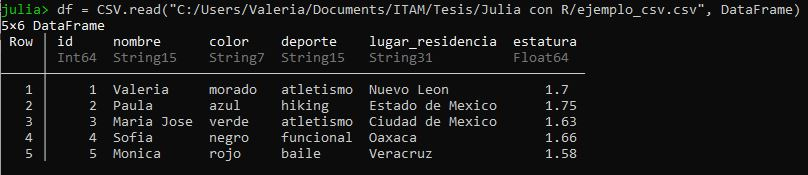
\includegraphics[scale=0.6]{Imagenes/insertar_df.PNG}
	\caption{Ejemplo de importación de un dataframe}
  \label{insertar_df}
\end{center}
\end{figure}

Los dataframes tienen una cantidad vasta de funciones que incluyen agregar o eliminar información, seleccionar columnas o renglones, transformar su contenido, etc. Las especificaciones de dichas funciones se explican con mayor profundidad en el manual oficial del paquete en la página \url{https://dataframes.juliadata.org/stable/}. 

\subsection{Análisis de regresión} \label{cap_regresiones}

El análisis de regresión es una herramienta estadística para estudiar las relaciones entre distintas variables. \say{Regresión es un método que permite a los investigadores resumir cómo predicciones o valores promedio de un resultado varían a través de variables individuales definidas como predictores o regresores}, \cite{regression_other_stories}. 

De forma concisa, la regresión es una expresión que intenta explicar como una variable depende de otras. En \textsf{Julia}, esto se puede hacer con ayuda del paquete \texttt{GLM} \citep{software_glm} que significa \textit{Generalized Linear Models} o modelos lineales generalizados. Una de sus funciones es ajustar modelos lineales, pero se puede usar para modelos más complejos. Como todos los paquetes, primero se debe instalar con los pasos descritos en la sección \ref{instalacion_paquete}. 

En este paquete una de las funciones principales se llama \texttt{lm} que se utiliza para ajustar un modelo lineal a un conjunto de datos. En el manual oficial \cite{glm_manual} se encuentra descrita la manera en que se pueden generar modelos más avanzados. Uno de los autores de este paquete, Douglas Bates tiene una larga trayectoria en el cómputo estadístico. En 1992 publicó el libro llamado \textit{Statistical Models in S} cuyo autor principal es John Chambers, otro grande del cómputo estadístico. Además, Bates es parte del llamado \textit{R Core Team} que es el grupo de colaboradores con acceso a la fuente del lenguaje \textsf{R}. Uno de sus trabajos más recientes es desarrollar modelos estadísticos en \textsf{Julia}, creando así el paquete \texttt{GLM}. 

La función \texttt{lm} se utiliza en repetidas ocasiones en este trabajo, por lo que se explica a continuación. La función es \texttt{lm(formula, data, allowrankdeficient=false; [wts::AbstractVector], dropcollinear::Bool=true)} donde 

\begin{itemize}
    \item \texttt{formula}: usa los nombres de las columnas del dataframe para referirse a las variables predictoras. Debe ser un objeto de tipo \texttt{formula}. 
    
    \item \texttt{data}: el dataframe que contenga los datos de los predictores de la fórmula.
    
    \item \texttt{allowrankdeficient}: de acuerdo al GitHub oficial del paquete\footnote{\url{https://github.com/JuliaStats/GLM.jl/blob/master/test/runtests.jl}}, este argumento está obsoleto y se recomienda utilizar \texttt{dropcollinear} en cambio. 
    
    \item \texttt{wts}: es un vector que especifica la ponderación de las observaciones. 
    
    \item \texttt{dropcolliinear}: controla si \texttt{lm} acepta una matriz que no sea de rango completo. Si el parámetro se define como \texttt{true} entonces solo se usan el conjunto de las primeras columnas linealmente dependientes.
\end{itemize}



\subsubsection{Regresión lineal simple}
El modelo de regresión lineal más simple es el que tiene un solo vector predictor $x$ y parámetros $a$ y $b$. 

\begin{equation*}
    \begin{aligned}
    y = a + bx + \epsilon.
    \end{aligned}
\end{equation*}

Para ejemplificar este modelo de regresión se usaron los datos del capítulo 7.1 del libro escrito por \cite{regression_other_stories}. La información fue recabada por Douglas Hibbs con el objetivo de predecir las elecciones de Estados Unidos basándose solamente en el crecimiento económico. Los datos se ven de la siguiente manera: 

\begin{figure}[H]
\begin{center}
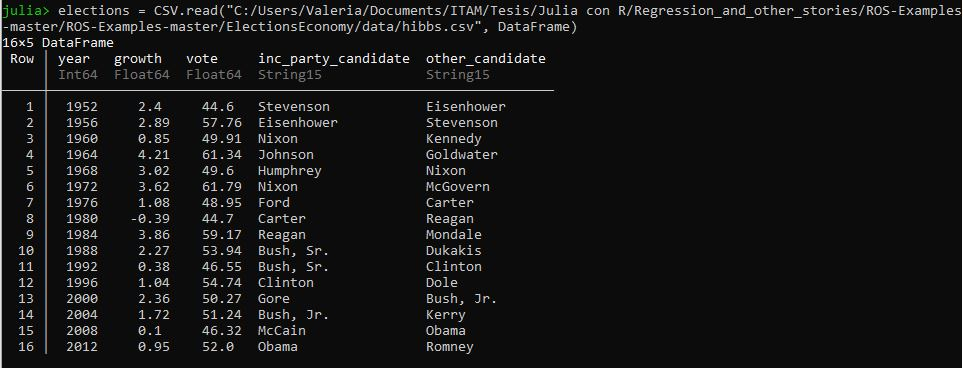
\includegraphics[scale=0.5]{Imagenes/elections_dataframe.PNG}
\caption{Encabezado de los datos sobre las elecciones en EUA recabados por Douglas Hibbs}
  \label{elections_dataframe}
\end{center}
\end{figure}

En este modelo se busca que el voto sea resultado del crecimiento económico. El código para hacer esto, después de la importación de datos mostrado en la figura \ref{elections_dataframe} es

\begin{minted}{julia}
	julia> elections_lm = 
	lm(@formula(vote ~ growth), elections)
\end{minted}

El resultado es una tabla con los coeficientes, su desviación estándar, el valor \textit{t}, el valor$-p$ y su intervalo de confianza del $95 \% $ como se muestra en la imagen \ref{ejemplo_rls}. En este ejemplo, el resultado que da \textsf{Julia} es \texttt{y = 46.2 + 3.1x}, el cual coincide con los valores reportados en el libro.

\begin{figure}[h]
	\begin{center}
		\includegraphics[scale=0.6]{Imagenes/ejemplo_rls.PNG}
		\caption{Ejemplo de regresión lineal simple en \textsf{Julia}}
		\label{ejemplo_rls}
	\end{center}
\end{figure}

\subsubsection{Regresión lineal múltiple}
La regresión lineal múltiple es el caso general de la regresión lineal simple. La diferencia es que en el primero hay múltiples predictores que deben cumplir ciertos criterios. \cite{regression_other_stories} define este tipo de regresión como 

\begin{equation*}
    \begin{aligned}
    y_i = \beta_0 + \beta_1 x_{i1} + \dots + \beta_k x_{ik} + \epsilon_i, \text{ para } i = 1, \dots, n
    \end{aligned}
\end{equation*}

\noindent donde $X_{ij}$ representa el $i$-ésimo regresor al $j$-ésimo nivel, los errores $\epsilon_i$ son independientes e idénticamente distribuidos de manera normal con media 0 y varianza $\sigma^2$. La representación matricial equivalente es 

\begin{equation} \label{eq_rlm}
    \begin{aligned}
        y_i = X_i \beta + \epsilon_i, \text{ para } i = 0, \dots, n
    \end{aligned}
\end{equation}

\noindent donde $X$ es una matriz de $(n+1) \times k$ cuyo renglón es $X_i$.

Para ejemplificar este tipo de modelo se usó un ejemplo que consta de dos predictores y la interacción entre ellos. Esta vez se utilizaron los datos del capítulo 10.3 de \cite{regression_other_stories} que muestran la relación entre los resultados de exámenes de niños (\texttt{kid\_score}), el coeficiente intelectual IQ de sus madres (\texttt{mom\_iq}) y si sus madres terminaron o no la preparatoria (\texttt{mom\_hs}). 

Se buscó determinar si existe una relación significativa entre la educación y el coeficiente de las madres con los resultados de los exámenes de sus hijos. Por lo tanto, los predictores son las variables en relación con la madre mientras que la respuesta es el desempeño de los niños. El código en \textsf{Julia} se ve de la siguiente manera

\begin{minted}{julia}
    julia> using DataFrames, GLM, CSV
    data_kid = CSV.read("~/Tesis/data/kidiq.csv", 
    	DataFrame)
    fm = @formula(kid_score ~ mom_hs + mom_iq)
\end{minted}

Que da como resultado el modelo ajustado

\texttt{kid\_score = 26 + 6* mom\_hs + 0.6*mom\_iq}

Uno de los aspectos por resaltar en este ejemplo es el uso del arroba representado con el carácter \texttt{@} antes de \texttt{formula}. El arroba se utiliza para llamar argumentos llamados macros en \textsf{Julia}. \texttt{formula} es una macro utilizada en el paquete \texttt{GLM}, por lo que el uso del arroba es indispensable. Las macros están fuera del alcance de este trabajo por lo que no se extenderá la explicación, pero en caso de requerir más información se sugiere buscar el apartado \textsf{Metaprogramming} en \cite{manual_Julia}. 

En el caso donde alguno de los regresores sea de tipo categórico, la fórmula se mantiene igual pero es necesario hacerle cambios a la base de datos en sí. Si \textsf{Julia} no reconoce estas columnas como categóricas entonces se debe cambiar su tipo en el dataframe. Se explica este caso más a fondo en el capítulo \ref{reg_categorias}. 

Por otro lado, se puede intentar usar el paquete \texttt{CSVFiles} para leer los archivos ya que hace mejor trabajo identificando el tipo de variables. Sin embargo, este paquete todavía está en desarrollo. 
